\subsubsection{Simulations for Fourier-Collocation Method}
	
	Following the same ideas from the previous section for Fourier-Collocation, we will seek solutions in the space given by $S_N = \widetilde{B}_N \cap H^2_p [0, 2 \pi]$, and using the discrete expansion to the problem (\ref{IVP_Burgers}) as follows
	\begin{align*}
		\mathcal{J}_N u (x, t) =  \displaystyle \sum_{|n| \leq \frac{N}{2}} \widetilde{u}_n (t) e^{inx}, \hspace{2mm}
		\widetilde{u}_n (t) =  \displaystyle \sum_{j=0}^{2N} u (x_j, t)  e^{-in x_j}
	\end{align*}
	or equivalently
	\begin{align*}
		\mathcal{J}_N u (x, t) =  \displaystyle \sum_{j=0}^{2N} u (x_j, t) \psi_j (x)
	\end{align*} 
	where $x_j$ are given by
	\begin{align*}
		xj = \frac{2 \pi j}{2N + 1}, \hspace{2mm} j = 0, 1, \dots, 2N.
	\end{align*}
	
	For this case, the Fourier-Collocation method will be given by the following problem
	\begin{align}
	\label{Collocation_Nonlinear}	
		R_{N} (x_j, t) = \frac{\partial u_N}{\partial t} (x_j, t) - \frac{\partial^2 u_N }{\partial x^2} (x_j, t) + \frac{1}{2} \frac{\partial \left[ u_N \right]^2}{\partial x} (x_j, t) = 0
	\end{align}
	which is a system of $2N + 1$ ordinary differential equations that can be solved using the initial condition given by
	\begin{align*}
		\mathcal{J}_N u (x_j, t) =  u_0 (x_j), , \hspace{2mm} j = 0, 1 \dots, 2N
	\end{align*}
	
	By Setting a vector as follows
	\begin{align*}
		u_N (t) &= (u_N (x_0 , t), u_N (x_1 , t), \dots , u_N (x_{2N} , t))^T,
	\end{align*} 
	and the above system of ordinary differential equations can be written as follows
	\begin{align*}
		\frac{d u_N (t)}{dt} =  \alpha D_N^2 u_N (t) - \frac{1}{2} D_N u^2_N (t)
	\end{align*}
	where $D_N$ is the matrix given by (\ref{matrix_DN_odd}), that represents discrete Fourier differentiation, which can be rewrite as
	\begin{align}
		D_N = \displaystyle C^{-1} \Lambda^2_N C
	\end{align}
	where $\Lambda_N = diag \{ ik \}_{|k|\leq N}$, $C$ represents the discrete Fourier transform and $C^{-1}$ the inverse. \\
	
	Note that the situation here is very different compared to the systems obtained with Fourier-Galerkin. The representation of the non-linear term is more practical to handle with implicit methods, for example, an implicit approach is as follows
	\begin{align*}
		u_N (t_{i + 1} ) =  C^{-1} \Lambda_N C u_N (t_{i}) - \frac{\Delta t}{2} D_N u^2_N (t_{i+1}) 
	\end{align*}
	
	It is possible to formulate the above problem as 
	\begin{align*}
		W(u_N (t_{i + 1})) =  C^{-1} \Lambda_N C u_N (t_{i}) - u_N (t_{i + 1} ) - \frac{\Delta t}{2} D_N u^2_N (t_{i+1}), 
	\end{align*}
	and then we must find $u_N(t_{i + 1})$ that satisfies $W(u_N(t_{i + 1})) = 0$, for example, using the Newton-Raphson method. However, this formulation may require many calculations because the differentiation matrix increases as a function of $N$, and therefore the number of operations. Here we are going to develop a numerical solution that is more practical to implement, implicitly approaching as we did with Fourier-Galerkin on the linear term as follows
	\begin{align*}
		\left[I_N + \frac{\Delta t}{2} u_{0} \Lambda_N \right] u_N (t_{i + 1} ) =  \displaystyle e^{-\Delta t \Lambda^0_N} \left[ u_N (t_{i}) - \frac{\Delta t}{2} D_N u^2_N (t_{i}) \right]
	\end{align*}
	where $\Lambda^0_N = diag \{ \alpha k^2 + \frac{ik}{2} u_0 \}_{|k|\leq N}$, and solving for $u_N (t_{i + 1})$ gives us
	\begin{align}
	\label{Collocation_Euler}	
		u_N (t_{i + 1} ) =  \displaystyle \left[I_N + \frac{\Delta t}{2} u_{0} \Lambda_N \right]^{-1} e^{-\Delta t \Lambda^0_N} \left[ u_N (t_{i})  - \frac{\Delta t}{2} D_N u^2_N (t_{i}) \right]
	\end{align}
	which is very similar to \ref{Galerkin_Euler}, except for the nonlinear term. \\
	  
	This formulation will be used for its implementation, and we will present some numerical results that were obtained using the same information that was used with Fourier-Galerkin, the difference is that the calculations are performed in real space using the differentiation matrix $D_N$, and in this case, we have the advantage of approximating the second derivative with $D^2_N = D_N \cdot D_N$. \\
	
	The description of the following results is as follows. In the figure \ref{Collocation_alphas} shows the maximum distance over every $t \in [0, 100]$ between the exact solution and its approximations given by (\ref{Collocation_Euler}) for $N = 2^m$, $m = 4, \dots, 12$, $\Delta t = 1.0 \times 10^{-5}$, and different values of $\alpha$. Furthermore, in Tables \ref{Collocation_tabla_L2_alpha=1} and \ref{Collocation_tabla_max_alpha=1}, we can see the numerical values ​​of these distances for different configurations of $N$ and $\Delta t$. Similarly, in Tables \ref{Collocation_tabla_L2_alpha=005} and \ref{Collocation_tabla_max_alpha=005} but for $\alpha = 0.005$.
	
	\newpage
	\begin{figure}[H]
		\centering
		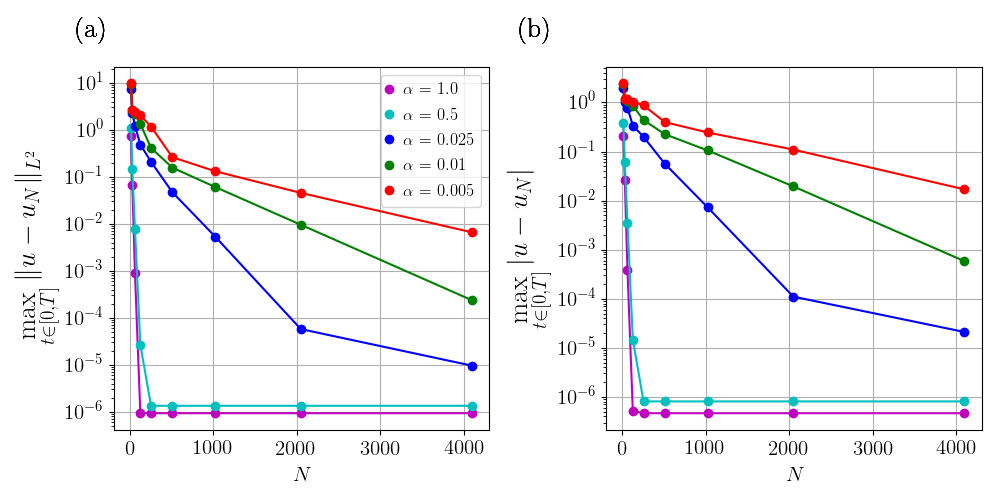
\includegraphics[width=12cm]{burgers_equation/deterministic/numerical_experiments/viscid/figures/collocation/alphas_Error_N.png}
		\caption{(a) $L^2$-norm between the exact solution and its approximations using Collocation method. (b) Max norm between the exact solution and its approximations.}
		\label{Collocation_alphas}
	\end{figure}

	\newpage
	\begin{figure}[H]
		\centering
		\caption{Numerical solution for (\ref{IVP_Burgers}) using (\ref{Collocation_Euler}) with $\alpha = 1.0$, $N=2048$, and $\Delta t = 1.0 \times 10^{-5}$.}
		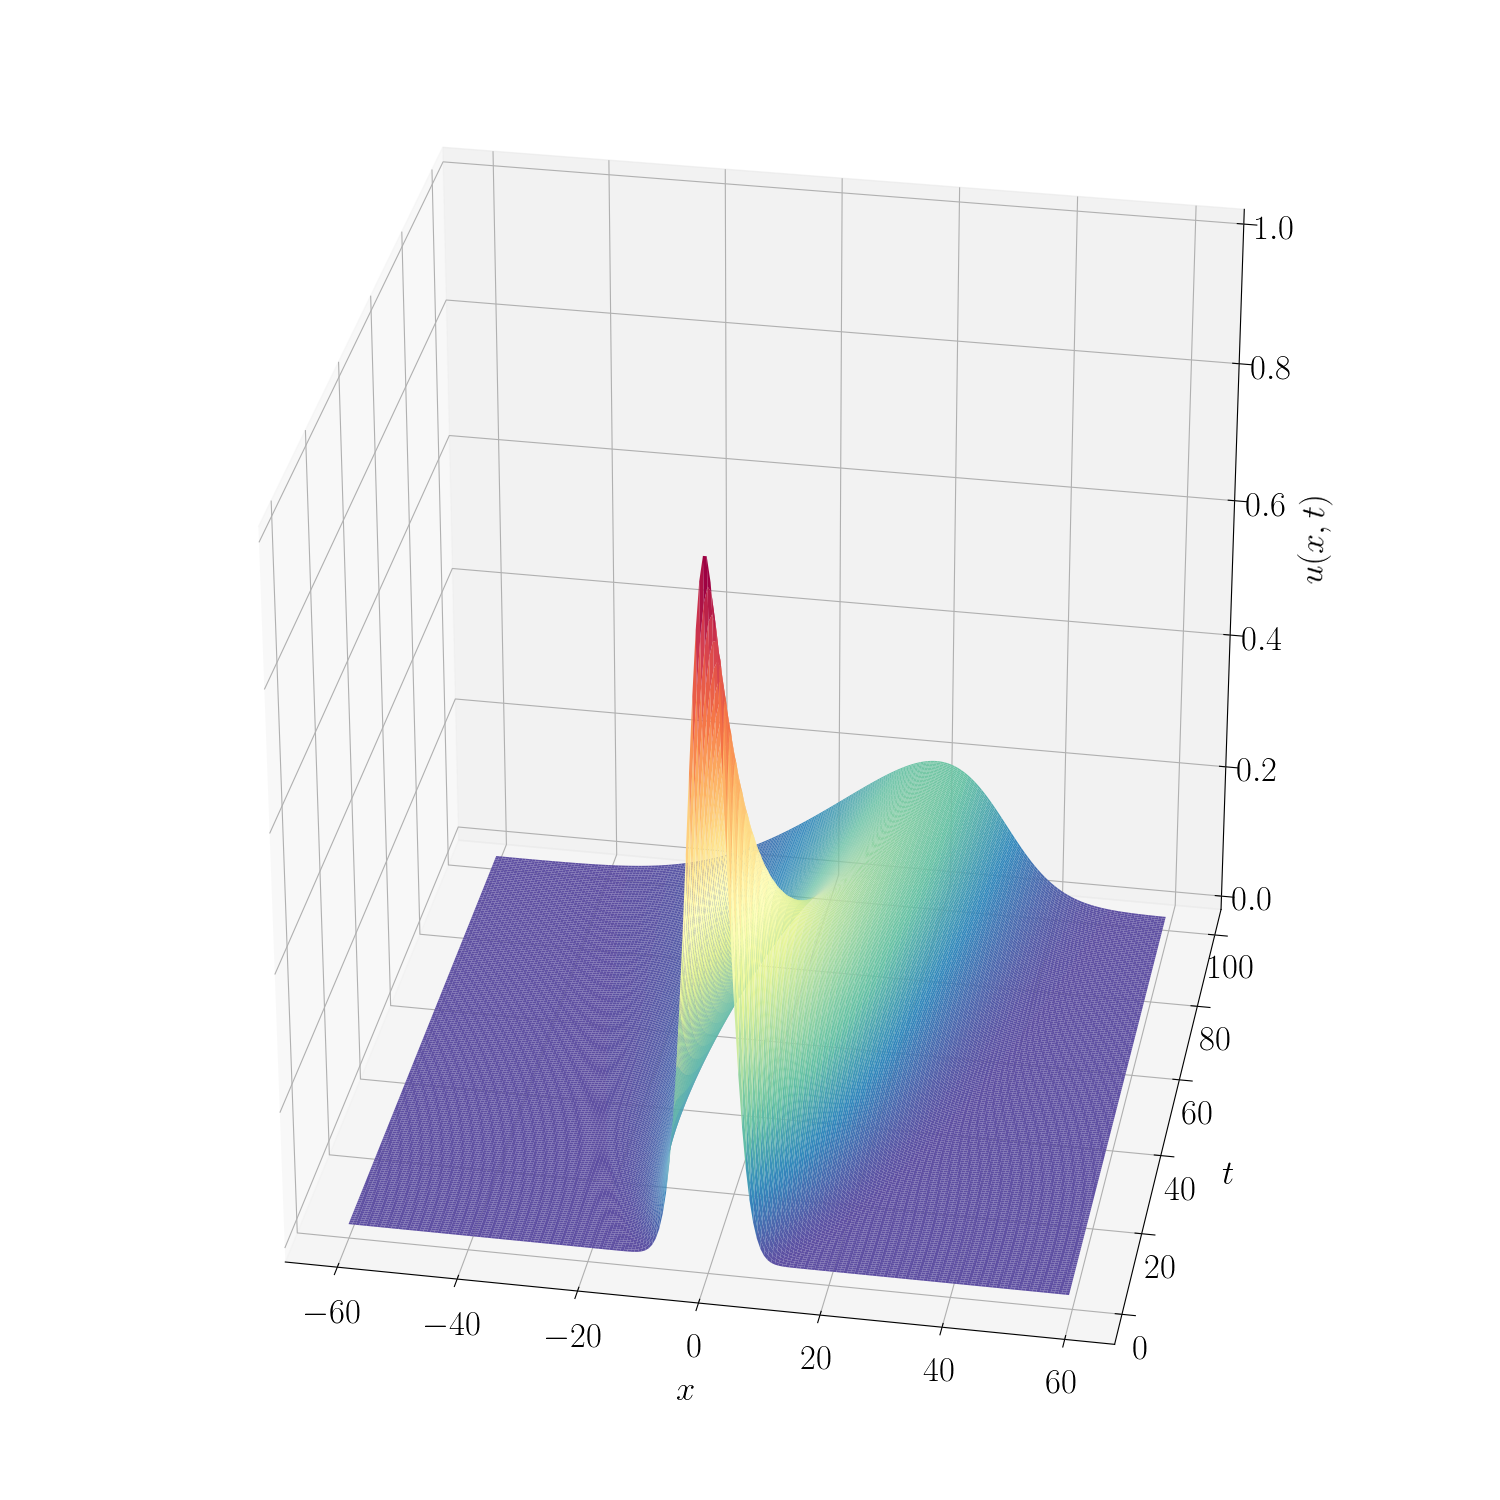
\includegraphics[width=12cm]{burgers_equation/deterministic/numerical_experiments/viscid/figures/collocation/Numerical_Solution_alpha=1.png}
		\label{Collocation_alpha=1}
		\caption{Numerical solution for (\ref{IVP_Burgers}) using (\ref{Collocation_Euler}) at the time $T = 100$ with $\alpha = 1.0$, and $\Delta t = 1.0 \times 10^{-5}$. (b) Point-wise error of approximation}
		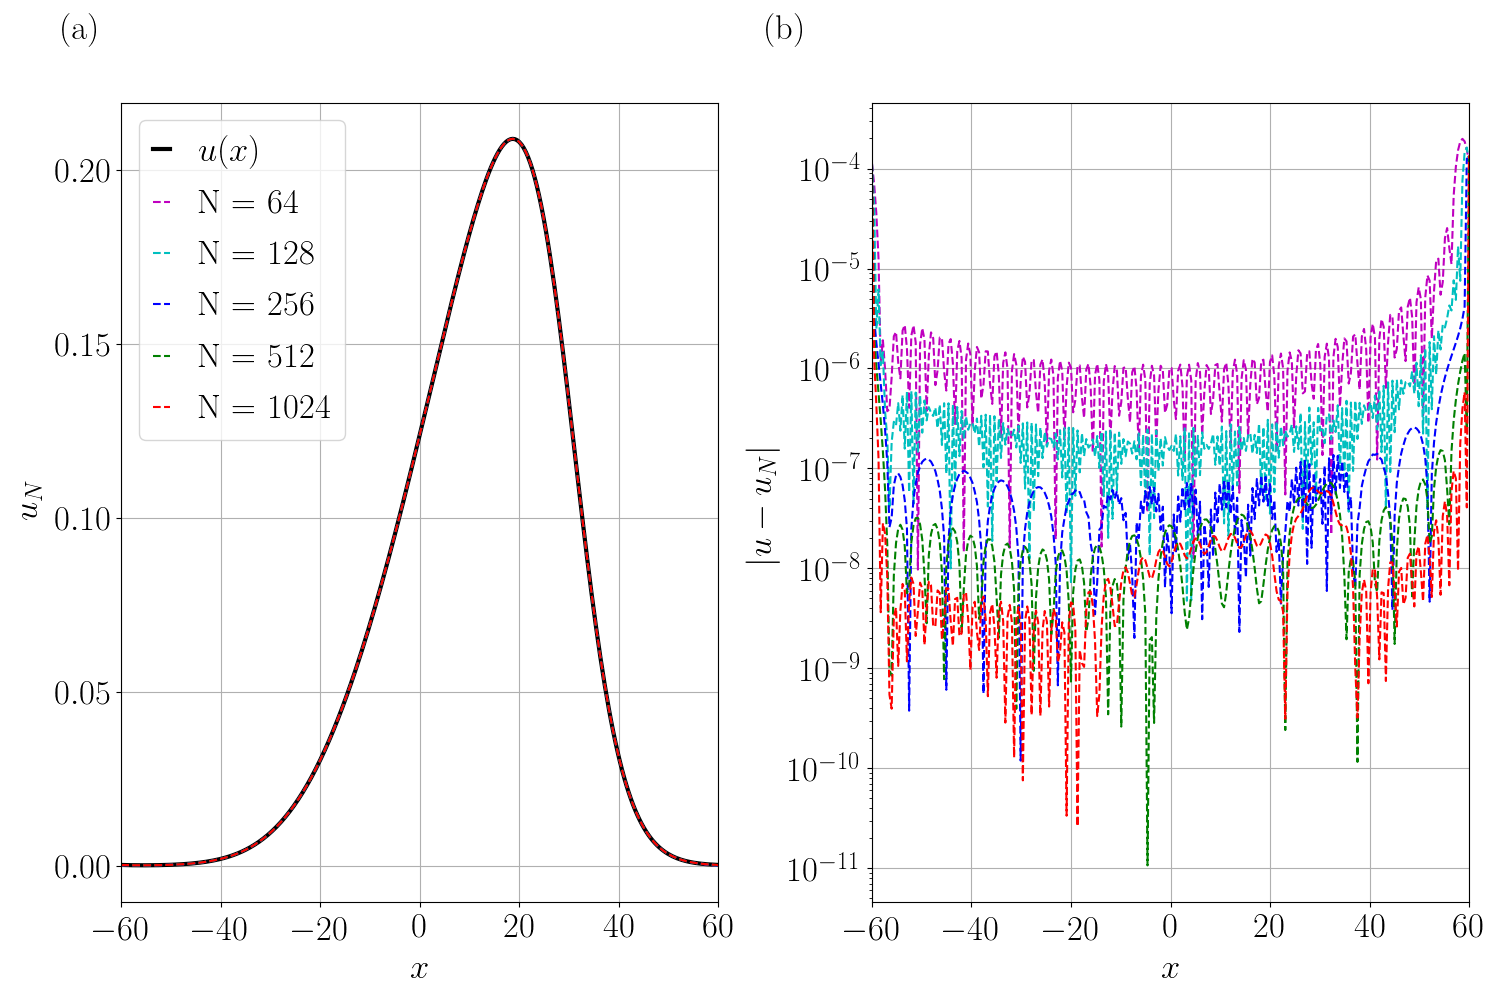
\includegraphics[width=12.5cm]{burgers_equation/deterministic/numerical_experiments/viscid/figures/collocation/Numerical_Solution_alpha=1_T=100.png}
		\label{Collocation_alpha=1_T}
	\end{figure}
	\begin{table}[H]
		\begin{tabular}{lcccc}
			\toprule
			\multicolumn{1}{c}{\textbf{Approximation}} & \multicolumn{4}{c}{\textbf{Error}} \\
			$\hspace{9mm}N$ & $\Delta t=1\times 10^{-2}$ & $\Delta t=1\times 10^{-3}$ & $\Delta t=1\times 10^{-4}$ & $\Delta t=1\times 10^{-5}$ \\
			\midrule
			\hspace{7mm} 16 & 0.721112    & 0.721112    & 0.721112    & 0.721112    \\
			\midrule
			\hspace{7mm} 32 & 4.71797 $\times 10^{-2}$   & 4.72892 $\times 10^{-2}$   & 4.73004 $\times 10^{-2}$   & 4.73015 $\times 10^{-2}$   \\
			\midrule
			\hspace{7mm} 64 & 1.17954 $\times 10^{-3}$  & 7.35344 $\times 10^{-4}$ & 7.27561 $\times 10^{-4}$ & 7.27283 $\times 10^{-4}$  \\
			\midrule
			\hspace{7mm} 128 & 9.43454 $\times 10^{-4}$ & 1.75152 $\times 10^{-4}$ & 1.74583 $\times 10^{-4}$ & 1.74574 $\times 10^{-4}$ \\
			\midrule
			\hspace{7mm} 256 & 9.43454 $\times 10^{-4}$ & 1.15509 $\times 10^{-4}$ & 1.14669 $\times 10^{-4}$ & 1.14659 $\times 10^{-4}$ \\
			\midrule
			\hspace{7mm} 512 & 9.43454 $\times 10^{-4}$ & 9.41793 $\times 10^{-5}$ & 7.78847 $\times 10^{-5}$ & 7.78707 $\times 10^{-5}$ \\
			\midrule
			\hspace{7mm} 1024 & $\ast$         & 9.41793 $\times 10^{-5}$ & 5.32213 $\times 10^{-5}$ & 5.32019 $\times 10^{-5}$ \\
			\midrule
			\hspace{7mm} 2048 & $\ast$           & $\ast$           & 3.56779 $\times 10^{-5}$ & 3.56498 $\times 10^{-5}$ \\
			\midrule
			\hspace{7mm} 4096 & $\ast$           & $\ast$           & 2.24122 $\times 10^{-5}$ & $\ast$           \\
			\\
			\bottomrule
		\end{tabular}
		\caption{Error using $L^2$-norm with $\alpha=1.0$}
		\label{Collocation_tabla_L2_alpha=1}
		\vspace{1cm}
		\begin{tabular}{lcccc}
			\toprule
			\multicolumn{1}{c}{\textbf{Approximation Max}} & \multicolumn{4}{c}{\textbf{Error}} \\
			$\hspace{9mm}N$ & $\Delta t=1\times 10^{-2}$ & $\Delta t=1\times 10^{-3}$ & $\Delta t=1\times 10^{-4}$ & $\Delta t=1\times 10^{-5}$ \\
			\midrule
			\hspace{7mm} 16 & 0.317617    & 0.317617    & 0.317617    & 0.317617    \\
			\midrule
			\hspace{7mm} 32 & 1.95279 $\times 10 ^{-2}$  & 1.96812 $\times 10 ^{-2}$   & 1.96965 $\times 10 ^{-2}$   & 1.96981 $\times 10 ^{-2}$   \\
			\midrule
			\hspace{7mm} 64 & 6.21793 $\times 10 ^{-4}$ & 2.9813 $\times 10 ^{-4}$  & 2.80086 $\times 10 ^{-4}$ & 2.78934 $\times 10 ^{-4}$ \\
			\midrule
			\hspace{7mm} 128 & 4.74952 $\times 10 ^{-4}$ & 1.64746 $\times 10 ^{-4}$ & 1.6473 $\times 10 ^{-4}$  & 1.64728 $\times 10 ^{-4}$ \\
			\midrule
			\hspace{7mm} 256 & 4.74936 $\times 10 ^{-4}$ & 1.52482 $\times 10 ^{-4}$ & 1.52467 $\times 10 ^{-4}$ & 1.52465 $\times 10 ^{-4}$ \\
			\midrule
			\hspace{7mm} 512 & 4.74936 $\times 10 ^{-4}$ & 1.47249 $\times 10 ^{-4}$ & 1.47234 $\times 10 ^{-4}$ & 1.47232 $\times 10 ^{-4}$ \\
			\midrule
			\hspace{7mm} 1024 & $\ast$           & 1.45032 $\times 10 ^{-4}$ & 1.45017 $\times 10 ^{-4}$ & 1.45016 $\times 10 ^{-4}$ \\
			\midrule
			\hspace{7mm} 2048 & $\ast$           & $\ast$           & 1.43941 $\times 10 ^{-4}$ & 1.4394 $\times 10 ^{-4}$ \\
			\midrule
			\hspace{7mm} 4096 & $\ast$           & $\ast$           & 1.43411 $\times 10 ^{-4}$ & $\ast$           \\
			\\
			\bottomrule
		\end{tabular}
		\caption{Error using Max norm with $\alpha=1.0$}
		\label{Collocation_tabla_max_alpha=1}
	\end{table}
	
	
	\begin{figure}[H]
		\centering
		\caption{Numerical solution for (\ref{IVP_Burgers}) using (\ref{Collocation_Euler}) with $\alpha = 0.005$, $N=2048$, and $\Delta t = 1.0 \times 10^{-5}$.}
		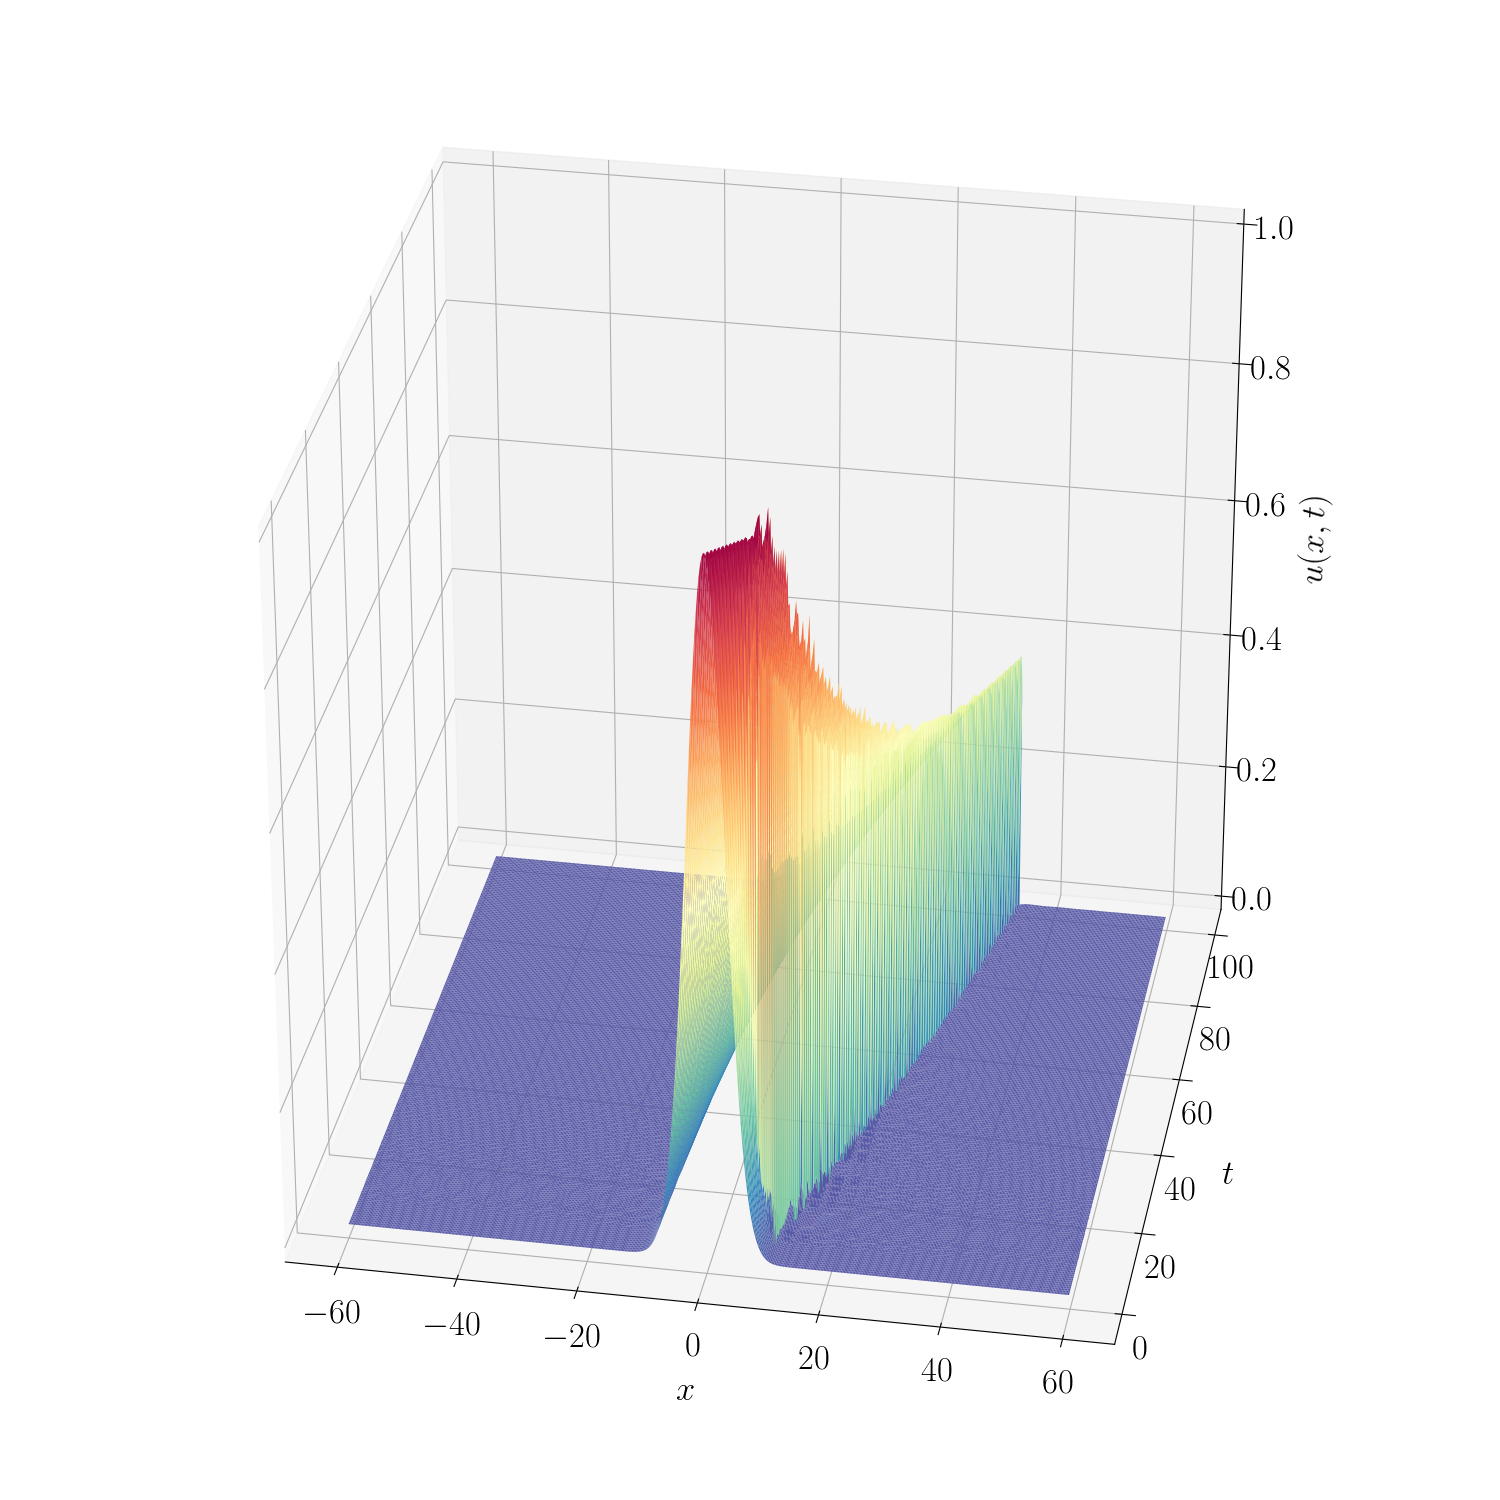
\includegraphics[width=12cm]{burgers_equation/deterministic/numerical_experiments/viscid/figures/collocation/Numerical_Solution_alpha=0005.png}
		\label{Collocation_alpha=005}
		\caption{Numerical solution for (\ref{IVP_Burgers}) using (\ref{Collocation_Euler}) at the time $T = 100$ with $\alpha = 0.005$, and $\Delta t = 1.0 \times 10^{-5}$. (b) Point-wise error of approximation.}
		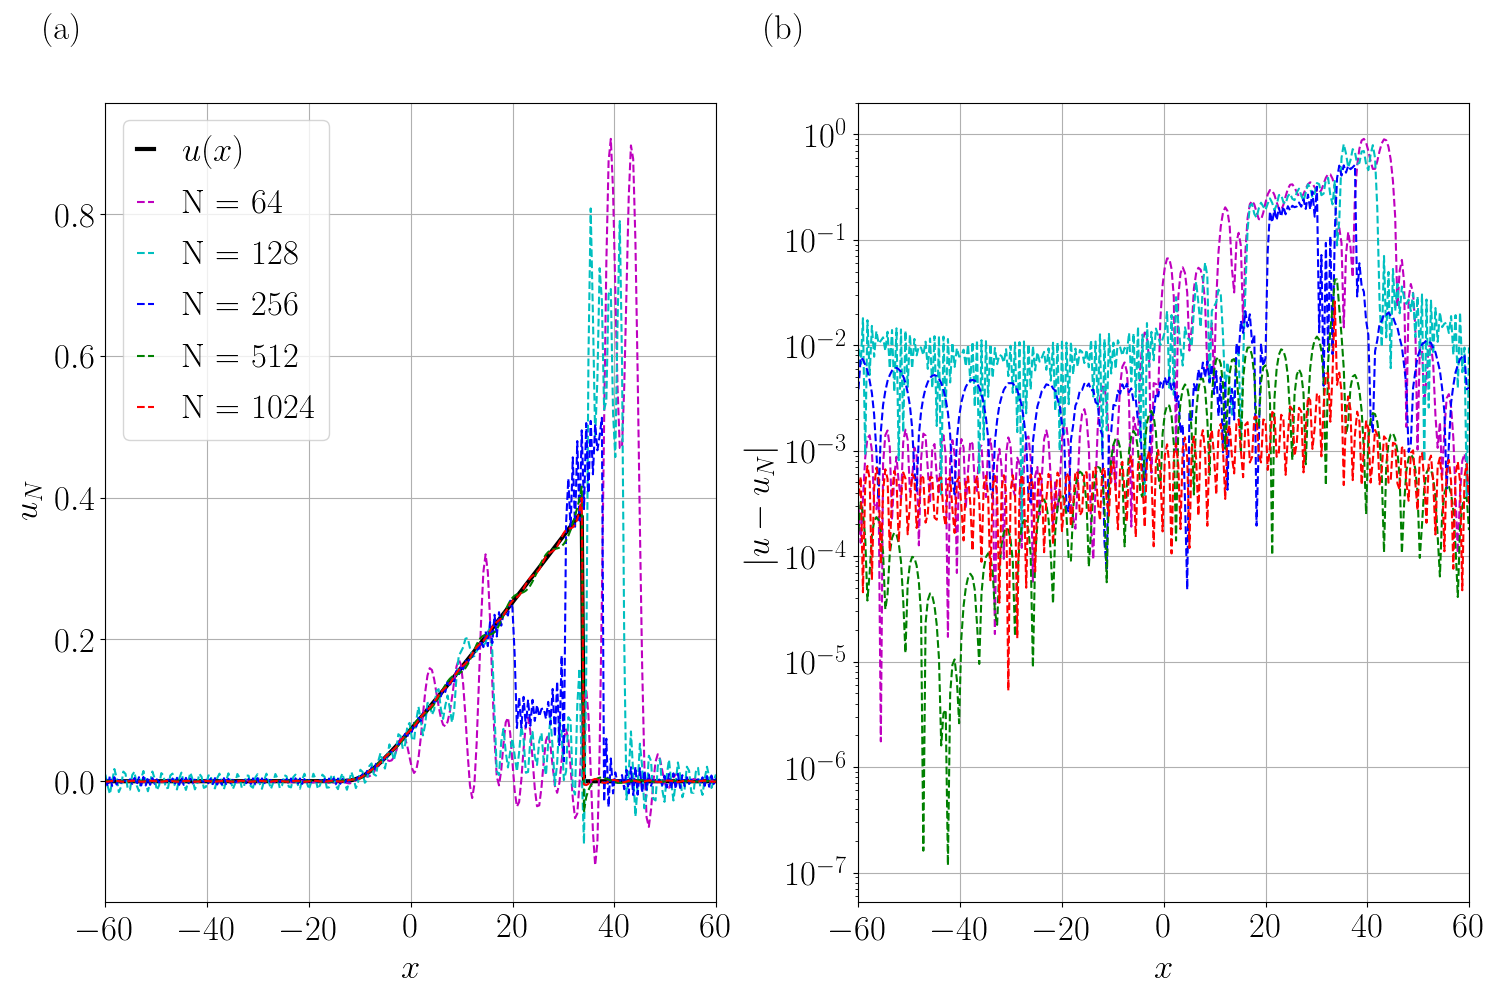
\includegraphics[width=12.5cm]{burgers_equation/deterministic/numerical_experiments/viscid/figures/collocation/Numerical_Solution_alpha=0005_T=100.png}
		\label{Collocation_alpha=005_T}
	\end{figure}
	%L2
	
	\begin{table}[H]
	\begin{tabular}{lcccc}
		\toprule
		\multicolumn{1}{c}{\textbf{Approximation}} & \multicolumn{4}{c}{\textbf{Error}} \\
		$\hspace{9mm}N$ & $\Delta t=1\times 10^{-2}$ & $\Delta t=1\times 10^{-3}$ & $\Delta t=1\times 10^{-4}$ & $\Delta t=1\times 10^{-5}$ \\
		\midrule
		\hspace{7mm} 16 & 1.36189   & 1.35883    & 1.35852   & 1.35849   \\
		\midrule
		\hspace{7mm} 32 & 2.67506   & 2.65305    & 2.65078   & 2.65055   \\
		\midrule
		\hspace{7mm} 64 & 2.50365   & 2.45855    & 2.45432   & 2.45387   \\
		\midrule
		\hspace{7mm} 128 & 2.15795   & 2.0632     & 2.05589   & 2.05497   \\
		\midrule
		\hspace{7mm} 256 & 1.362     & 1.18393    & 1.16697   & 1.16532   \\
		\midrule
		\hspace{7mm} 512 & 0.350775  & 0.304595   & 0.300865  & 0.300499  \\
		\midrule
		\hspace{7mm} 1024 & 0.168462  & 0.140332   & 0.13803   & 0.137804  \\
		\midrule
		\hspace{7mm} 2048 & 6.56161 $\times 10^{-2}$ & 4.63808 $\times 10^{-2}$  & 4.49226 $\times 10^{-2}$ & 4.47813 $\times 10^{-2}$ \\
		\midrule
		\hspace{7mm} 4096 & $\ast$         & 7.66246 $\times 10^{-3}$ & 6.9909 $\times 10^{-3}$ & 6.9909 $\times 10^{-3}$         \\
		\\
		\bottomrule
	\end{tabular}
	\caption{Error using $L^2$-norm with $\alpha=0.005$}
	\label{Collocation_tabla_L2_alpha=005}
	\vspace{1cm}
	\begin{tabular}{lcccc}
		\toprule
		\multicolumn{1}{c}{\textbf{Approximation Max}} & \multicolumn{4}{c}{\textbf{Error}} \\
		$\hspace{9mm}N$ & $\Delta t=1\times 10^{-2}$ & $\Delta t=1\times 10^{-3}$ & $\Delta t=1\times 10^{-4}$ & $\Delta t=1\times 10^{-5}$ \\
		\midrule
		\hspace{7mm} 16 & 0.695784 & 0.695659  & 0.695646  & 0.695645 \\
		\midrule
		\hspace{7mm} 32 & 1.20278  & 1.19418   & 1.19329   & 1.1932   \\
		\midrule
		\hspace{7mm} 64 & 1.22454  & 1.18903   & 1.18507   & 1.18467  \\
		\midrule
		\hspace{7mm} 128 & 1.11999  & 1.0238    & 1.01754   & 1.01701  \\
		\midrule
		\hspace{7mm} 256 & 0.927954 & 0.877058  & 0.872508  & 0.87201  \\
		\midrule
		\hspace{7mm} 512 & 0.664133 & 0.415288  & 0.39714   & 0.395563 \\
		\midrule
		\hspace{7mm} 1024 & 0.247742 & 0.259451  & 0.260605  & 0.26072  \\
		\midrule
		\hspace{7mm} 2048 & 0.126824 & 0.103297  & 0.107102  & 0.10748  \\
		\midrule
		\hspace{7mm} 4096 & $\ast$        & 2.04624 $\times 10 ^{-2}$ & 1.76513  $\times 10 ^{-2}$ & 1.76513  $\times 10 ^{-2}$        \\
		\\
		\bottomrule
	\end{tabular}
	\caption{Error using Max norm with $\alpha=0.005$}
	\label{Collocation_tabla_max_alpha=005}
	\end{table}